
Вывод уравнения фильтрации основан на следующих предположениях: 
\begin{itemize}
	\item пласт однородный и изотропный - пористость и проницаемость одинаковы во всем пласте и во всех направлениях и не зависят от давления 
	\item добывающая скважина вскрывает весь продуктивный горизонт и обеспечивает радиальный приток к скважине
	\item пласт насыщен одним флюидом на всем протяжении
	\item температура не меняется в пласте, изотермичность
\end{itemize}

Схема притока приведена на рисунке \ref{ris:radial_inflow_scheme}.

\begin{figure}[h!]
	\begin{center}
		

\tikzset{every picture/.style={line width=0.75pt}} %set default line width to 0.75pt        

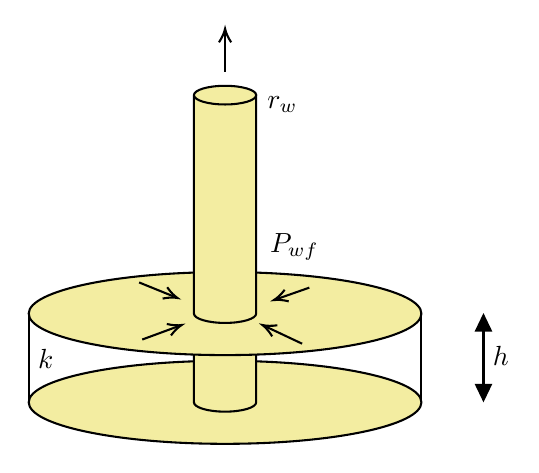
\begin{tikzpicture}[x=0.75pt,y=0.75pt,yscale=-1,xscale=1]
%uncomment if require: \path (0,300); %set diagram left start at 0, and has height of 300

%Shape: Ellipse [id:dp024533754320974488] 
\draw  [fill={rgb, 255:red, 243; green, 237; blue, 161 }  ,fill opacity=1 ] (255.9,210) .. controls (255.9,198.95) and (298.25,190) .. (350.5,190) .. controls (402.75,190) and (445.1,198.95) .. (445.1,210) .. controls (445.1,221.05) and (402.75,230) .. (350.5,230) .. controls (298.25,230) and (255.9,221.05) .. (255.9,210) -- cycle ;
%Shape: Can [id:dp18120956683853207] 
\draw  [fill={rgb, 255:red, 243; green, 237; blue, 161 }  ,fill opacity=1 ] (365.5,176.25) -- (365.5,210) .. controls (365.5,212.49) and (358.78,214.5) .. (350.5,214.5) .. controls (342.22,214.5) and (335.5,212.49) .. (335.5,210) -- (335.5,176.25) .. controls (335.5,173.76) and (342.22,171.75) .. (350.5,171.75) .. controls (358.78,171.75) and (365.5,173.76) .. (365.5,176.25) .. controls (365.5,178.74) and (358.78,180.75) .. (350.5,180.75) .. controls (342.22,180.75) and (335.5,178.74) .. (335.5,176.25) ;
%Shape: Ellipse [id:dp0014041786513778742] 
\draw  [fill={rgb, 255:red, 243; green, 237; blue, 161 }  ,fill opacity=1 ] (255.9,167.25) .. controls (255.9,156.2) and (298.25,147.25) .. (350.5,147.25) .. controls (402.75,147.25) and (445.1,156.2) .. (445.1,167.25) .. controls (445.1,178.3) and (402.75,187.25) .. (350.5,187.25) .. controls (298.25,187.25) and (255.9,178.3) .. (255.9,167.25) -- cycle ;
%Shape: Can [id:dp09417665438601963] 
\draw  [fill={rgb, 255:red, 243; green, 237; blue, 161 }  ,fill opacity=1 ] (365.5,62) -- (365.5,167.25) .. controls (365.5,169.74) and (358.78,171.75) .. (350.5,171.75) .. controls (342.22,171.75) and (335.5,169.74) .. (335.5,167.25) -- (335.5,62) .. controls (335.5,59.51) and (342.22,57.5) .. (350.5,57.5) .. controls (358.78,57.5) and (365.5,59.51) .. (365.5,62) .. controls (365.5,64.49) and (358.78,66.5) .. (350.5,66.5) .. controls (342.22,66.5) and (335.5,64.49) .. (335.5,62) ;
%Straight Lines [id:da05427875829374096] 
\draw    (255.9,167) -- (255.9,210) ;
%Straight Lines [id:da08444018377929519] 
\draw    (445.1,167) -- (445.1,210) ;
%Straight Lines [id:da7446827946920336] 
\draw    (475,170) -- (475,207) ;
\draw [shift={(475,210)}, rotate = 270] [fill={rgb, 255:red, 0; green, 0; blue, 0 }  ][line width=0.08]  [draw opacity=0] (8.93,-4.29) -- (0,0) -- (8.93,4.29) -- cycle    ;
\draw [shift={(475,167)}, rotate = 90] [fill={rgb, 255:red, 0; green, 0; blue, 0 }  ][line width=0.08]  [draw opacity=0] (8.93,-4.29) -- (0,0) -- (8.93,4.29) -- cycle    ;
%Straight Lines [id:da9533475438509436] 
\draw    (309.1,152.25) -- (325.75,159) ;
\draw [shift={(327.6,159.75)}, rotate = 202.07] [color={rgb, 255:red, 0; green, 0; blue, 0 }  ][line width=0.75]    (6.56,-2.94) .. controls (4.17,-1.38) and (1.99,-0.4) .. (0,0) .. controls (1.99,0.4) and (4.17,1.38) .. (6.56,2.94)   ;
%Straight Lines [id:da7628148018069294] 
\draw    (310.6,179.75) -- (327.72,173.44) ;
\draw [shift={(329.6,172.75)}, rotate = 519.78] [color={rgb, 255:red, 0; green, 0; blue, 0 }  ][line width=0.75]    (6.56,-2.94) .. controls (4.17,-1.38) and (1.99,-0.4) .. (0,0) .. controls (1.99,0.4) and (4.17,1.38) .. (6.56,2.94)   ;
%Straight Lines [id:da8513852103635728] 
\draw    (387.6,181.75) -- (370.31,173.6) ;
\draw [shift={(368.5,172.75)}, rotate = 385.23] [color={rgb, 255:red, 0; green, 0; blue, 0 }  ][line width=0.75]    (6.56,-2.94) .. controls (4.17,-1.38) and (1.99,-0.4) .. (0,0) .. controls (1.99,0.4) and (4.17,1.38) .. (6.56,2.94)   ;
%Straight Lines [id:da03702921414833504] 
\draw    (391.1,154.75) -- (375.89,160.09) ;
\draw [shift={(374,160.75)}, rotate = 340.66999999999996] [color={rgb, 255:red, 0; green, 0; blue, 0 }  ][line width=0.75]    (6.56,-2.94) .. controls (4.17,-1.38) and (1.99,-0.4) .. (0,0) .. controls (1.99,0.4) and (4.17,1.38) .. (6.56,2.94)   ;
%Straight Lines [id:da15593017089479355] 
\draw    (350.5,50.67) -- (350.5,32) ;
\draw [shift={(350.5,30)}, rotate = 450] [color={rgb, 255:red, 0; green, 0; blue, 0 }  ][line width=0.75]    (6.56,-2.94) .. controls (4.17,-1.38) and (1.99,-0.4) .. (0,0) .. controls (1.99,0.4) and (4.17,1.38) .. (6.56,2.94)   ;

% Text Node
\draw (258.9,182.73) node [anchor=north west][inner sep=0.75pt]    {$k$};
% Text Node
\draw (370.67,126.98) node [anchor=north west][inner sep=0.75pt]    {$P_{wf}$};
% Text Node
\draw (478,181.73) node [anchor=north west][inner sep=0.75pt]    {$h$};
% Text Node
\draw (369.33,61.07) node [anchor=north west][inner sep=0.75pt]    {$r_{w}$};


\end{tikzpicture}
		\caption{Схема радиального притока к скважине}
		\label{ris:radial_inflow_scheme}
	\end{center}
\end{figure}

Используются следующие обозначения параметров:

\(h\) - толщина пласта

\(k\) - средняя проницаемость

\(r\) - радиус (расстояние от скважины)

\(r_e\) -  внешний радиус зоны дренирования

\(r_w\) - радиус скважины

\(p\) - давление

\(q\) - объемный расход флюида в рабочих условиях - дебит

\(t\) - время

\(u_r\) - приведенная скорость

\(\varphi\) -  пористость

\(\mu\) - вязкость

\(\rho\) - плотность флюида

\subsubsection{Радиальная модель притока}
Уравнение фильтрации или уравнение движения флюидов основывается на принципах сохранения массы и импульса (количества движения). Для жидкости закон сохранения импульса принимает форму закона Дарси. При этом эффекты турбулентности и отклонения потока от Дарси не учитываются. Они важны для газовых скважин и могут быть введены в уравнение фильтрации отдельно. 

Закон сохранения массы или принцип неразрывности можно выразить в радиальной форме следующим соотношением

\begin{equation} \label{eq:mass_balance_2}
\frac{1}{r}\frac{\partial\left(r\rho u_r\right)}{\partial r}=-\varphi\frac{\partial p}{\partial t}
\end{equation}

Принцип неразрывности показывает, что для определенного объема пласта, масса флюида которое втекла в контрольный объем пласта минус масса которая вытекла равна массе которая накопилась в объеме. 

Сохранение импульса или закон Дарси можно выразить соотношением  


\begin{equation} \label{eq:darcy_law_2}
 u_r=-\frac{k}{\mu}\frac{d^p}{dr}
\end{equation}

Закон Дарси здесь используется как псевдоустановившаяся аппроксимация обобщенного уравнения сохранения импульса (то есть слагаемым отвечающим за накопление импульса пренебрегаем). Это предположение справедливо если не учитывать возмущения давления в среде двигающиеся со скоростью звука. Все изменения давления описываемые моделью связаны с локальными изменениями градиента давления за счет ламинарного режима потока. Хотя далее в модели будет учтена сжимаемость системы всеми "звуковыми" \ эффектами в системе мы пренебрегаем.

Поток предполагается горизонтальным, поэтому давление \( p\) может быть использовано в качестве потенциала потока, гравитационными силами пренебрегаем.

Комбинируя уравнения (\ref{eq:mass_balance_2}), (\ref{eq:darcy_law_2})  получим:

\begin{equation} \label{eq:diff_eq_2}
\frac{1}{r}\frac{\partial\left( \dfrac{r\rho k}{\mu}\dfrac{\partial p}{dr}\right)}{\partial r}=\varphi\frac{\partial \rho}{\partial t}
\end{equation}

Уравнение (\ref{eq:diff_eq_2}) -- дифференциальное уравнение в частных производных описывающее нестационарный поток однофазного флюида в пористой среде при ламинарном потоке. 

Вообще говоря приведенное уравнение является нелинейным, так как плотность $\rho = \rho(p)$ и вязкость $\mu = \mu(p)$ являются функциями давления. Уравнение содержит две зависимые переменные - давление $p$ и плотность $\rho$. Поэтому для его решения необходимо задать еще одно соотношение, каковым может быть уравнение состояния флюида связывающее плотность флюида и давление $\rho = \rho(p)$. 

\subsubsection{Флюид постоянной сжимаемости}
 
Нестационарное поведение давления в пласте связано со сжимаемостью системы. При изменении давления в какой то точке, часть флюида сжимается, происходит накопление или отдача флюида, что вызывает задержку в распространении изменения флюида. Несмотря на то, что сжимаемость флюидов и породы малы и во многих случаях ими можно пренебречь, это не верно для пластовых систем для добычи нефти. Большие объемы пласта и флюидов и высокие давления компенсируют малость сжимаемости и требуют ее учета. 

Для однофазного флюида разумным является предположение постоянства сжимаемости.

Сжимаемость можно определить как 

$$c=-\frac{1}{V} \left(  \frac{ \partial V}{ \partial p}  \right) $$ 

учтем, что

$$ \rho = \frac{m}{V} $$  

тогда получим

$$c=\frac{1}{\rho} \left(  \frac{ \partial \rho}{ \partial p}  \right) $$ 

Для флюида с постоянной сжимаемостью, проинтегрировав приведенное уравнение можно получить 

$$\rho = \rho_i e^{c(p-p_i)}$$

где $\rho_i$ плотность флюида при некотором заданном давлении $p_i$

Продифференцировав выражение для плотность по времени получим 

$$
c \rho \frac{\partial p}{\partial t} = \frac{\partial \rho}{\partial t}
$$

Подставив это выражение в ранее полученное уравнение фильтрации получим 

$$ 
\frac{1}{r}\frac{\partial\left( \dfrac{r\rho k}{\mu}\dfrac{\partial p}{dr}\right)}{\partial r}=\varphi c \rho \frac{\partial p}{\partial t}  
$$

Приведенное дифференциальное уравнение в частных производных все еще нелинейно, поскольку зависит от плотности $\rho$ 



\subsubsection{Общая сжимаемость}
Если пористость не является постоянной величиной и меняется с давлением, тогда  слагаемое отвечающее за накопление флюида в пласте можно выразить как 


$$\frac{\partial \varphi \rho}{\partial t} = \varphi \frac{\partial \rho}{\partial t}+ \rho \frac{\partial \varphi }{\partial t} = \varphi c_l \rho \frac{\partial p}{\partial t} + \rho \frac{\partial \varphi }{\partial t}  $$

где $c_l$ сжимаемость жидкости. 

Определим сжимаемость породы как 

$$c_f = \frac{1}{\varphi} \frac{\partial \varphi}{\partial p}$$

тогда 

$$\frac{\partial \varphi \rho}{\partial t}  = \varphi \rho (c_l + c_f) \frac{\partial p}{\partial t}   $$



хотя пористость здесь является функцией давления - в первом приближении мы можем считать ее константой равной пористости при некотором среднем давлении в пласте. Это справедливо для маленькой сжимаемости породы, что верно почти всегда.

Уравнение для сжимаемости можно еще уточнить, учтя что в пласте могут находится различные флюиды - вода и нефть с насыщенностями  $s_w$ и $s_o$

тогда 

$$ c_l = s_o c_o + s_w c_w $$

тогда можно ввести общую сжимаемость системы 

$$ c_t = c_l + c_f = s_o c_o + s_w c_w  + c_f $$ 

Заметим, что проницаемость k в законе Дарси это не абсолютная проницаемость, но относительная проницаемость по нефти при насыщенности водой соответствующей связанной воде.  

$$ k= k_o (s_{wc}) $$

\subsubsection{Линеаризация уравнения фильтрации}

Раскрыв производную в левой части уравнения и предположив, что $\dfrac{\partial p}{\partial r}$ мало а следовательно слагаемым  $ r \rho c_t \left( \dfrac{\partial p}{\partial r} \right)^2 $ можно пренебречь, что приведет к линеаризации уравнения фильтрации

\begin{equation} \label{eq:diff_eq_lin}
\frac{\partial^2 p}{\partial r^2} + \frac{1}{r} \frac{\partial p}{\partial r}= \frac{\varphi \mu c_t}{k} \frac{\partial p}{\partial t}
\end{equation}

